% Copyright 2020 by Robert Hildebrand
%This work is licensed under a
%Creative Commons Attribution-ShareAlike 4.0 International License (CC BY-SA 4.0)
%See http://creativecommons.org/licenses/by-sa/4.0/

\documentclass[border=0.1cm]{standalone}
\usepackage{tikz,amsmath,amssymb}
\usetikzlibrary{positioning}


\begin{document}


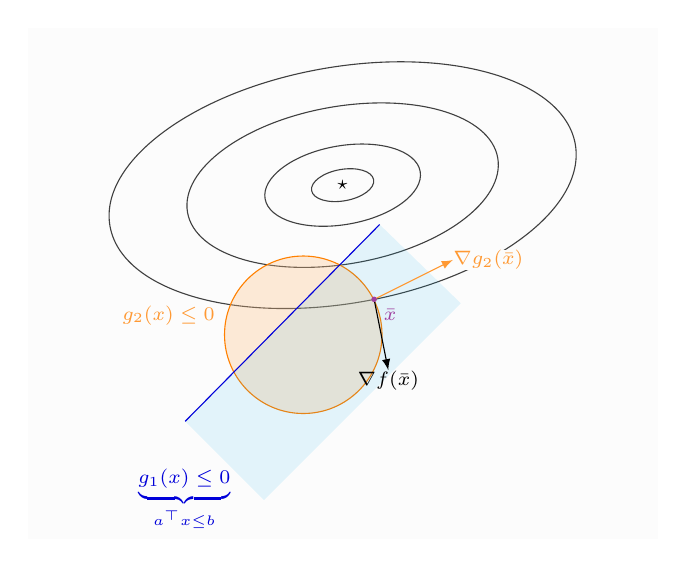
\begin{tikzpicture}
\fill[black!1] (-4,-4.5) rectangle (4,2);
\begin{scope}[rotate=10]
\draw[black!75,] (0,0) ellipse(.4cm and 0.2cm) node[black]{\scriptsize $\star$};
\draw[black!75] (0,0) ellipse(1cm and 0.5cm);
\draw[black!75] (0,0) ellipse(2cm and 1cm);
\draw[black!75] (0,0) ellipse(3cm and 1.5cm);
\end{scope}

\draw[fill=orange!50,draw=orange,fill opacity=0.3, text opacity=1] (-.5,-1.9) circle(1cm) node[above left=0cm and 1cm,color=orange!80]{\scriptsize $g_2(x)\leq 0$};
\fill[cyan,fill opacity=0.1, text opacity=1] (-2,-3) -- (0.47,-.5) -- (1.5, -1.5) -- (-1,-4)node[left=0.3cm,blue!85!black]{\scriptsize $\underbrace{g_1(x)\leq0}_{a^\top x\leq b}$} -- cycle ;
\draw[blue!85!black] (-2,-3) -- (0.47,-.5); 
%\fill[violet!75] (-.035,-1.01) circle(1pt);
%\draw[blue!85!black,-latex] (-1.75,-2.75) -- ++ (-0.5,.5) node[left]{\scriptsize $\nabla g_1(x)=a$};

\node at (0.4,-1.45) (x) {};
%\draw[blue!85!black,-latex,xshift=1.17cm,yshift=1.2cm] (-1.75,-2.75) -- ++ (-0.8,.8) node[left,fill=black!1,inner sep=0]{\scriptsize $\nabla g_1(\bar{x})$};
\draw[color=orange!80,-latex] (0.4,-1.45) -- ++ (1,.5) node[right,fill=black!1,inner sep=0]{\scriptsize $\nabla g_2(\bar{x})$};
%\draw[black,-latex,xshift=1.17cm,yshift=1.2cm] (-1.75,-2.75) -- ++ (0,.9) node[above,fill=black!1,inner sep=0]{\scriptsize $-\nabla f(\bar{x})$};
\draw[black,-latex] (0.4,-1.45) -- ++ (.18,-.9) node[below,inner sep=0]{\scriptsize $\nabla f(\bar{x})$};

%\fill[violet!75] (-.035,-1.01) circle(1pt) node[below]{\scriptsize $\bar{x}$};
%\fill[violet!99] (-.58,-1.56) circle(1pt)  node[below right]{\scriptsize $\bar{x}$};
\fill[violet!75] (0.4,-1.45) circle(1pt) node[below right]{\scriptsize $\bar{x}$};


\end{tikzpicture}

\end{document}
